\documentclass[11pt,a4paper]{moderncv}
\moderncvtheme[blue]{classic}
\usepackage[utf8]{inputenc}
\usepackage[top=0.6cm, bottom=0.6cm, left=0.7cm, right=0.7cm]{geometry}
\usepackage[english]{babel}
\setlength{\hintscolumnwidth}{3.5cm} % width of the left column (dates)
%\setlength{\makecvtitlenamewidth}{20cm}

\firstname{Romain}
\familyname{Pellerin}
\title{Software Engineering Student}
%\photo[54pt][0.0pt]{picture} % '64pt' is the height the picture must be resized to, 0.0pt is the thickness of the frame around it (put it to 0pt for no frame) and 'picture' is the name of the picture file
\address{Currently living in San Francisco}{\textbf{Open to relocation}}{} % street, city, country
\email{contact@romainpellerin.eu}
\homepage{romainpellerin.eu}
\mobile{+1 415-937-4830}
%\mobile{+33 6 95 60 57 81}
\extrainfo{\href{https://github.com/rpellerin}{github.com/rpellerin}}
\quote{Objective: a full-time job from September 2017}
\renewcommand*{\quotefont}{\Large\bfseries} % override quote's default style

% I took the original code from moderncvstylebanking.sty and changed line 25
% USEFUL for theme banking
% \makeatletter
% \renewcommand*{\maketitle}{%
%   \setlength{\maketitlewidth}{1.0\textwidth}%
%   \hfil%
%   \parbox{\maketitlewidth}{%
%     \centering%
%     % name and title
%     \namestyle{\@firstname~\@lastname}%
%     \ifthenelse{\equal{\@title}{}}{}{\titlestyle{~|~\@title}}\\% \isundefined doesn't work on \@title, as LaTeX itself defines \@title (before it possibly gets redefined by \title)
%     % detailed information
%     \addressfont\color{color2}%
%     \ifthenelse{\isundefined{\@addressstreet}}{}{\addtomaketitle{\addresssymbol\@addressstreet}%
%       \ifthenelse{\equal{\@addresscity}{}}{}{\addtomaketitle[~--~]{\@addresscity}}% if \addresstreet is defined, \addresscity and \addresscountry will always be defined but could be empty
%       \ifthenelse{\equal{\@addresscountry}{}}{}{\addtomaketitle[~--~]{\@addresscountry}}%
%       \flushmaketitle\@firstmaketitleelementtrue\\}%
%     \collectionloop{phones}{% the key holds the phone type (=symbol command prefix), the item holds the number
%       \addtomaketitle{\csname\collectionloopkey phonesymbol\endcsname\collectionloopitem}}%
%     \ifthenelse{\isundefined{\@email}}{}{\addtomaketitle{\emailsymbol\emaillink{\@email}}}%
%     \ifthenelse{\isundefined{\@homepage}}{}{\addtomaketitle{\homepagesymbol\httplink{\@homepage}}}%
%     \collectionloop{socials}{% the key holds the social type (=symbol command prefix), the item holds the link
%       \addtomaketitle{\csname\collectionloopkey socialsymbol\endcsname\collectionloopitem}}%
%     \ifthenelse{\isundefined{\@extrainfo}}{}{\addtomaketitle{\@extrainfo}}%
%     \flushmaketitle}\\[2.5em]}% need to force a \par after this to avoid weird spacing bug at the first section if no blank line is left after \maketitle
%  \makeatother

\begin{document}
\makecvtitle

\section{Education}
\cventry{2014 -- present}{Diplôme d'ingénieur en informatique (Software engineering degree)}{\href{http://www.utc.fr/formations-enseignements/genie-informatique.php}{Université de Technologie de Compiègne}}{Compiègne (France)}{Expected August 2017}{} % year, degree, institution, city+picture = {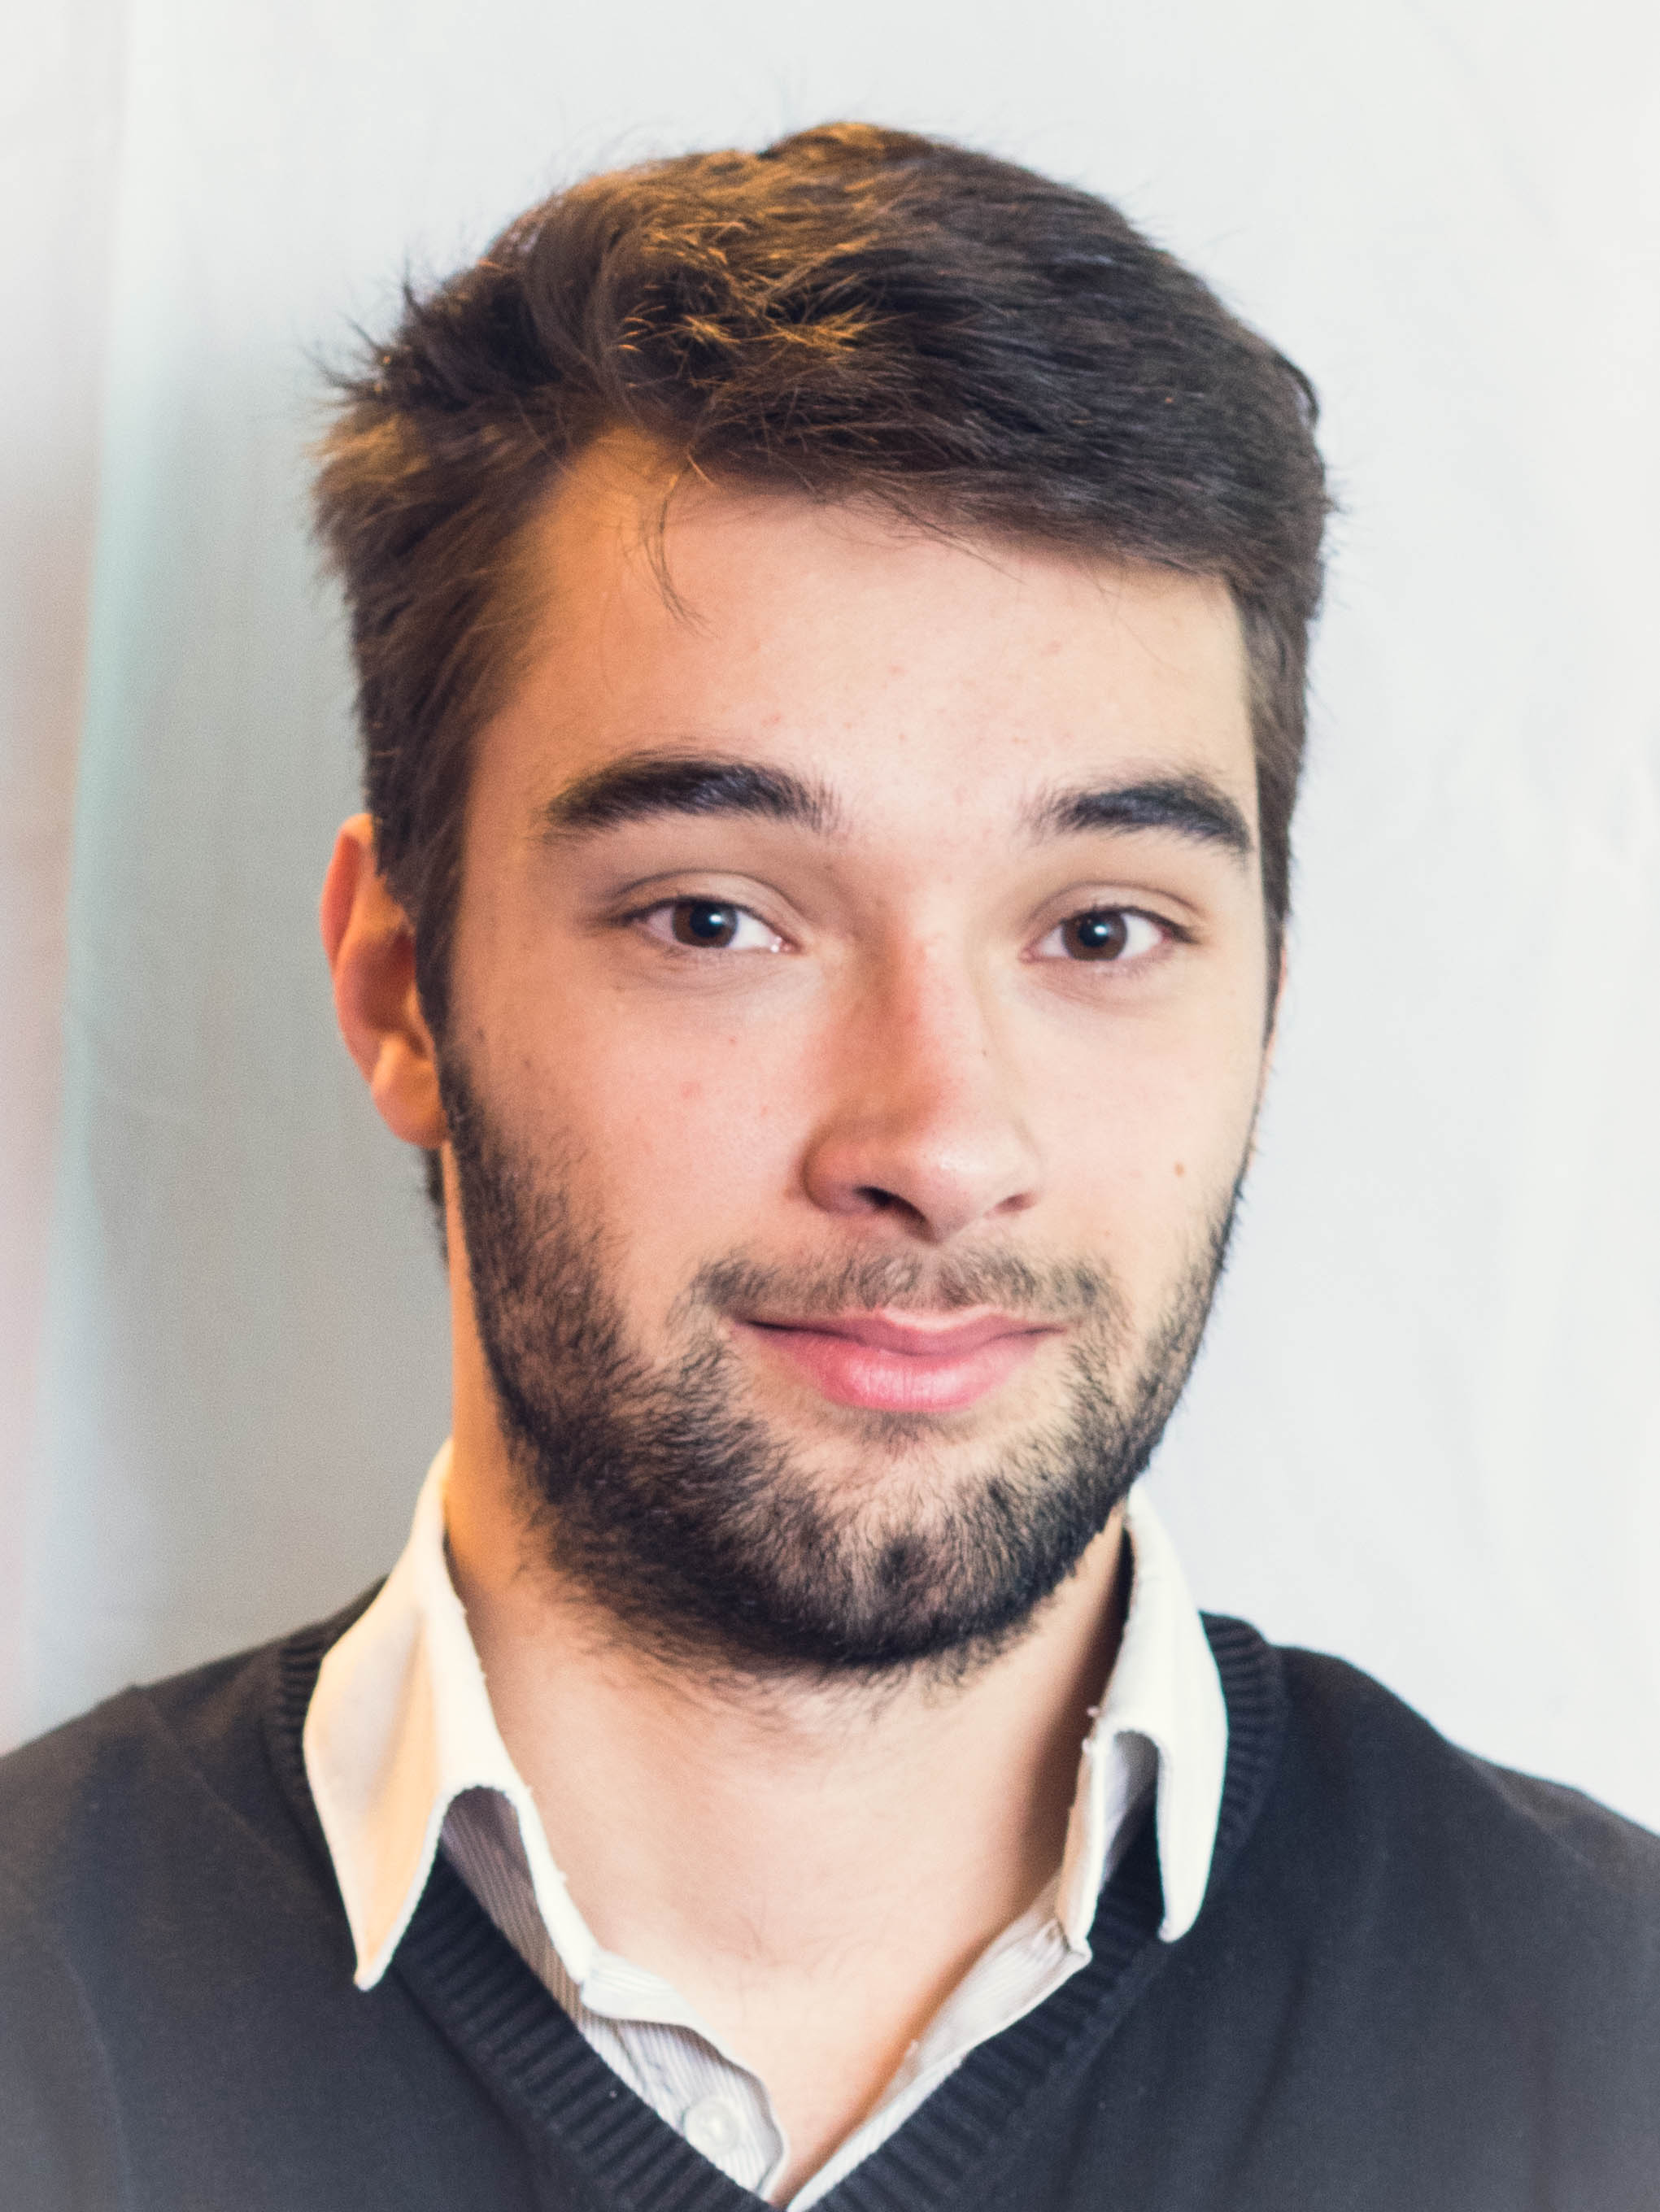
\includegraphics[scale=0.5]{picture}City}, grade, description
\cventry{2016}{Exchange program (Fall semester)}{\href{http://www.kaist.ac.kr/html/en/}{KAIST}}{Daejeon (South Korea)}{}{} % year, degree, institution, city+picture = {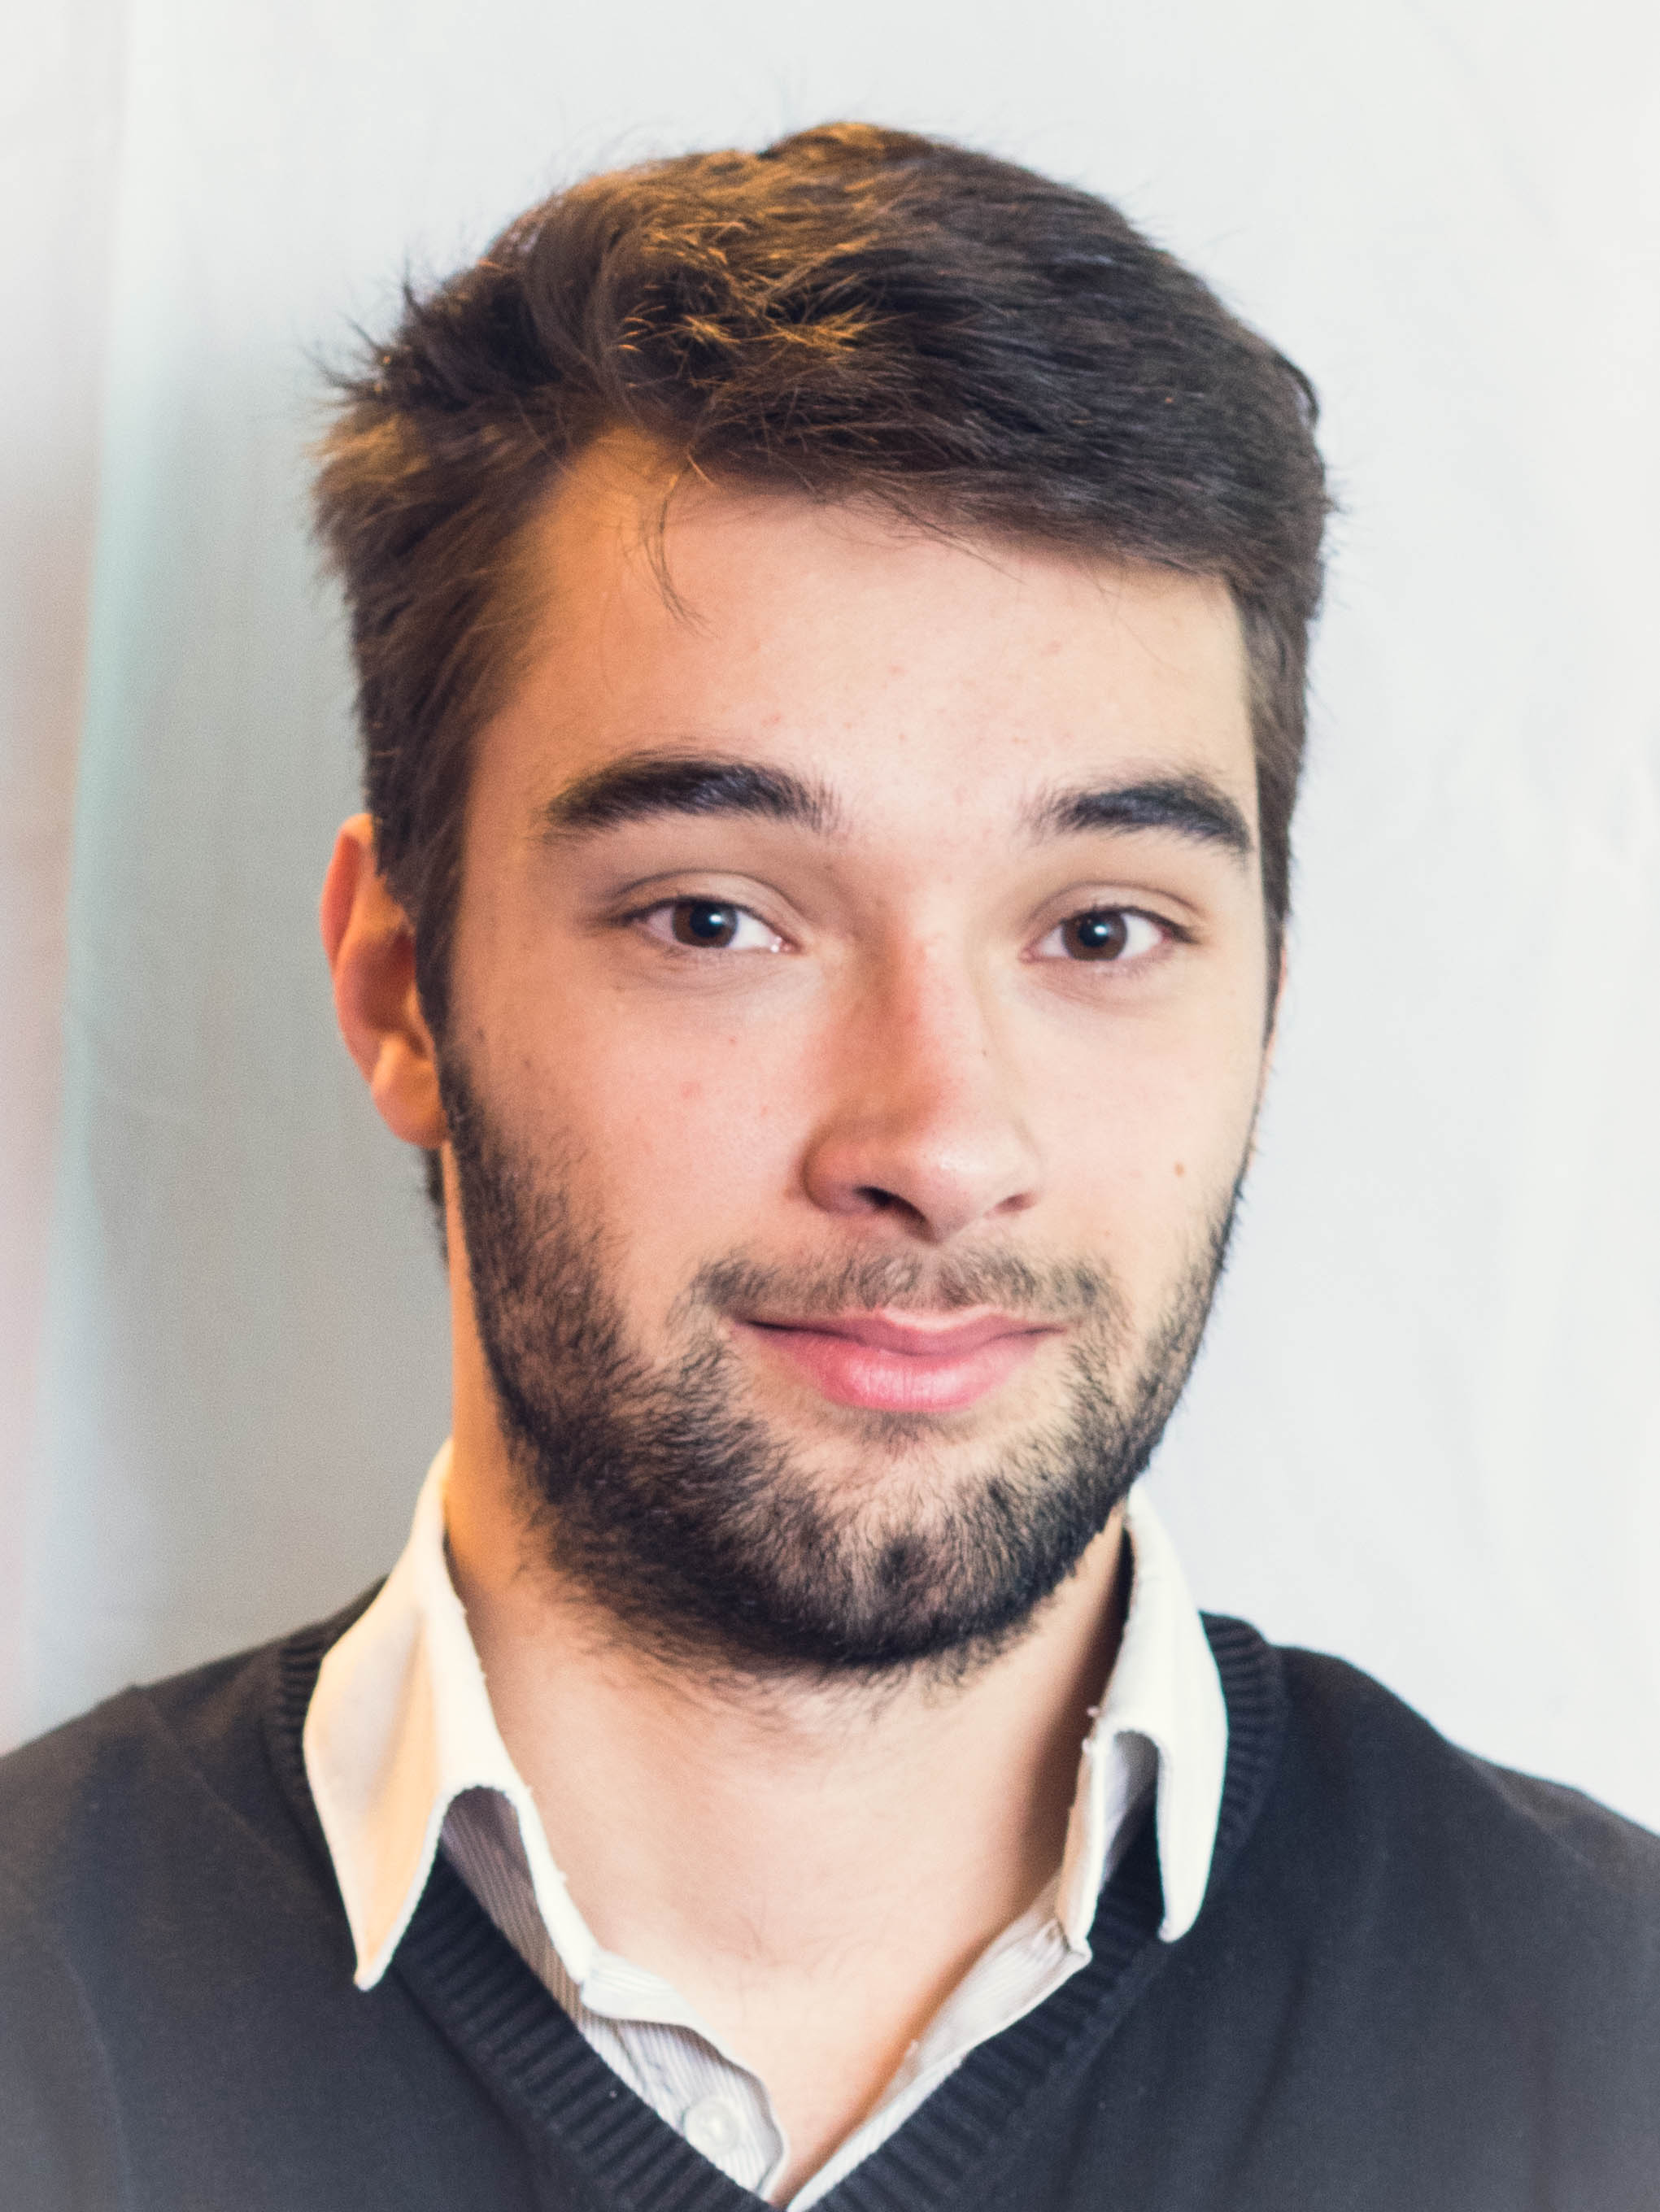
\includegraphics[scale=0.5]{picture}City}, grade, description
\cventry{2012 -- 2014}{DUT Informatique (Two-year university degree in Computer Science)}{\href{http://www.iutnantes.univ-nantes.fr/321/0/fiche___formation/}{Institut Universitaire de Technologie de Nantes}}{Nantes (France)}{}{}

\section{Professional Experience}
\cventry{Feb 2017 -- Jul 2017}{Intern in software development}{\href{http://inovia.fr/}{Inovia Team}}{San Fransisco (USA)}{}{asm.js and WebAssembly.}
\cventry{Sep 2015 -- Feb 2016}{Intern in mobile application development}{\href{http://www.wearesmiths.com/}{The Smiths}}{Amsterdam (The Netherlands)}{}{Developed Android and iOS applications with the Titanium framework).
\begin{itemize}
  \item Front-end with the following frameworks: Backbone, Underscore, Titanium/Alloy
  \item Back-end with Express, hosted on \href{http://www.parse.com/}{parse.com}; also some SQL and Shell scripting
\end{itemize}}
\cventry{Sep 2014 -- Jun 2015}{Computer Science Manager}{\href{http://www.usec-utc.fr/}{USEC}}{Compiègne (France)}{}{In charge of software development projects for local companies.
\begin{itemize}
  \item Wrote official documents (quotes, specifications, customer agreements, etc.)
  \item Recruited and mentored students (those who develop our clients' projects)
\end{itemize}}
\cventry{Jun 2013 -- Sep 2014}{Android and web developer}{Self-employed}{Nantes (France)}{}{Developed and then updated the Android application and the website of the startup \textsc{\href{http://www.who-wanna.com/en/}{WhoWanna}}.}%\newline{}
\cventry{Apr 2014 -- Jun 2014}{Intern in software development}{\href{http://www.who-wanna.com/en/}{WhoWanna}}{Nantes (France)}{}{
\begin{itemize}%
\item Updated the Android application (added some features, graphical update)
\item Also: PHP, MySQL, PostgreSQL, and a bit of Scala
\end{itemize}}

\section{Volunteer Experience}
\cventry{Mar 2015 -- Jun 2015}{President and co-organizer of tech talks}{\href{https://www.youtube.com/playlist?list=PL3nMxbEwNq0wE3BNx5b0EEtp8h-yvHyIy}{HumanTalks}}{Compiègne (France)}{}{10-minute talks given once a month about programming languages, tools, software development, etc\\\href{http://humantalks.com/cities/compiegne}{http://humantalks.com/cities/compiegne}}

\section{Computer Skills}
% \cvcomputer{category}{programs}{category}{programs}
% \cvdoubleitem{subtitle}{text}{subtitle}{text}
\cvitem{Languages}{\textbf{JavaScript (familiar with ES6), Java, PHP, HTML, CSS}, Python, Bash, C++ (Qt)}
\cvitem{Databases}{\textbf{PostgreSQL, MySQL}, SQLite (+ UML as a modeling language)}
\cvitem{OSes}{\textbf{GNU/Linux} (\href{http://xubuntu.org/}{Xubuntu} as my main OS, based on Debian)}
\cvitem{Other}{\textbf{Git, Apache2}, system administration (iptables, fail2ban, OpenVPN, TCP/IP), \LaTeX}

\section{Languages}
\cvlanguage{French}{Native speaker}{}
\cvlanguage{English}{Full professional proficiency -- European C1/C2 level}{\textbf{TOEIC 985/990 (March 2016)}}

\section{Hobbies}
\cvdoubleitem{\textbf{Raspberry Pi:}}{Websites, VPN, ownCloud}{\textbf{Side-projects:}}{Android apps, web browser add-ons}
\cvdoubleitem{\textbf{Conferences:}}{I gave talks and attended some, such as \href{http://devfest.gdgnantes.com/}{DevFest} or \href{http://web2day.co/}{Web2Day}}{\textbf{Free software:}}{Supporter; most of my source code is on \href{https://github.com/rpellerin}{GitHub}}
\cvdoubleitem{\textbf{Music:}}{I have been playing the guitar for fifteen years}{\textbf{Sport:}}{Workout, cycling}
\end{document}
